\documentclass[11pt]{article}
\usepackage[margin=1.0in]{geometry}
\addtolength{\topmargin}{0.25in}
\usepackage[document]{ragged2e}
\usepackage{graphicx}
\graphicspath{{../pictures/}}
\usepackage{float}
\usepackage{siunitx}


\begin{document}
	{\Huge\textbf{EEE381 Tech Memo}}\\
	\hfill \break
	\textbf{From:} Charles Noah Lutz\\
	\textbf{Partner:} Aaron Smith, Mitchell Darnell\\
	\textbf{To:} Colin Bussert\\
	\textbf{Date:} Performed: 10/18/18; Due: 10/27/18\\
	\textbf{Subject:} Lab \#03

	\section{Abstract}
	The purpose of this exercise was to build two current sources, one
	simple current source using two transistors and the other a modified
	Wilson current source, using four transistors and to observe and
	analyze the differences between them.
	
	\section{Theory}
	MOSFETs can be used to make a current source to supply a certain amount of
	current to a cicuit. In this exercies two different current sources were 
	built and compared. The first was a simple current source using two transistors.
	The circuit can be seen in Figure \ref{fig:simple}.

	\begin{figure}[H]
		\centering
		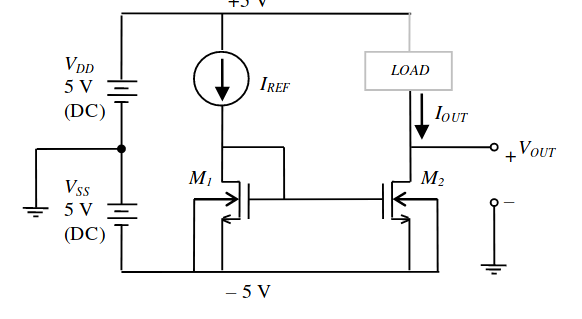
\includegraphics[width=4.0 in]{simple_current.png}
		\caption{Simple current source}
		\label{fig:simple}
	\end{figure}

	The reference current, $I_{ref}$ is created using a resistor. The current 
	through the resistor depends only on the value of that resistor. This 
	relationship can be seen in Equation \ref{equ:simple_rref}.

	\begin{equation}
		\label{equ:simple_rref}
		R_{ref} = \frac{2V_{DD} - V_{GS}}{I_D}
	\end{equation}
	
	Since the target current for this exercise was 4 $\si{\milli\ampere}$,
	$R_{ref}$ can be calculated using $V_{DD}$, $V_{SS}$, and the transistor 
	current equation. Using this method, the calculated $R_{ref}$ for 4 
	$\si{\milli\ampere}$ current was 1637 \si\ohm. It should be noted that 
	because there is no manufactured resistor with this value, the closest
	value resistor was used, which was 1.5 $\si{\kilo\ohm}$.\\

	\hfill \break

	The second current source that was built was a modified Wilson current
	source. This source uses four transistors and can be seen in Figure
	\ref{fig:mod_wilson}.

	\begin{figure}[H]
		\centering
		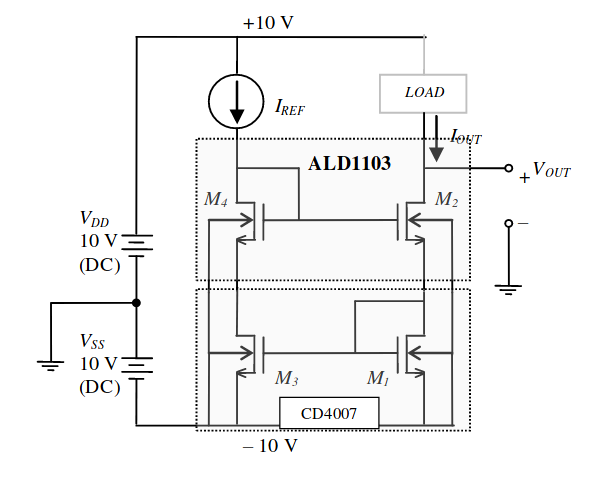
\includegraphics[width=4.0 in]{m_wilson_current.png}
		\caption{Modified Wilson current source}
		\label{fig:mod_wilson}
	\end{figure}

	Just as with the simple current source, $I_{ref}$ is created using a
	resistor, $R_{ref}$. The equation for this resistor, however is slightly
	different due to the fact that there are two voltage drops down to 
	$V_{SS}$ through two transistors. This means that the $V_{GS}$ term must
	be multiplied by two. This can be seen in Equation \ref{equ:wilson_rref}.

	\begin{equation}
		\label{equ:wilson_rref}
		R_{ref} = \frac{2V_{DD} - 2V_{GS}}{I_D}
	\end{equation}

	Again, using this equation and the transitor current equation, the calculated
	value of $R_{ref}$ is 3275 $\si\ohm$. It should be noted that no resistors are
	manufactured at this value and therefore, the resistor that was actually used
	was a 3.3 $\si{\kilo\ohm}$.\\

	\hfill \break

	When comparing these two current sources, an important property to look
	at is the output impedance. The output impedance of the simple current 
	source is simply the output impedance of the transistor, $r_o$ while the
	output impedance of the Wilson current source is $g_m r_o^2$. This makes
	the Wilson current source closer to an ideal current source since the 
	output impeadance of an ideal current source is ininity. Using the given
	properties of the transistors, the $R_{out}$ for the simple current source
	is 25 $\si{\kilo\ohm}$ and the $R_{out}$ for the Modified Wilson current
	source is 2.5 $\si{\mega\ohm}$.\\

	

	\hfill \break

	Both the current sources have a maximum load resistatnce that they can
	drive. If the resistance becomes too large, the current through the load
	will drop below the reference current due to the transistor falling out 
	of saturation. This can be calculated using the transistor current equations
	and the conditions for saturation. Table \ref{table:max_res} shows the max
	resistances for each current source.

	\begin{table}[H]
		\centering
		\caption{Maximum Load Resistance}
		\label{table:max_res}
		\begin{tabular}{|c|c|}
			\hline
			Current Source & $R_{L_{max}} (\si\ohm)$\\
			\hline
			Simple & 1987\\
			\hline
			Modified Wilson & 3900\\
			\hline
		\end{tabular}
	\end{table}

	Both cirucit were simulated using PSPICE to observe the effect that 
	changing the load resistance had on the current through the current
	source. The data for both the simple and Wilson current source can
	be seen in Tables \ref{table:simple_pspice} and \ref{table:wilson_pspice}.

	\begin{table}[H]
		\centering
		\caption{Simple Current Source $I_D$ vs. $R_L$}
		\label{table:simple_pspice}
		\begin{tabular}{|c|c|}
			\hline
			$R_L$ (\si\ohm) & $I_D (\si{\milli\ampere})$\\
			\hline
			100 & 3.78\\
			500 & 3.75\\
			1000 & 3.70\\
			1500 & 3.64\\
			2000 & 3.55\\
			2500 & 3.30\\
			\hline
		\end{tabular}
	\end{table}

	\begin{table}[H]
		\centering
		\caption{Wilson Current Source $I_D$ vs. $R_L$}
		\label{table:wilson_pspice}
		\begin{tabular}{|c|c|}
			\hline
			$R_L$ (\si\ohm) & $I_D (\si{\milli\ampere})$\\
			\hline
			100 & 3.58\\
			1000 & 3.56\\
			1500 & 3.55\\
			2000 & 3.55\\
			2500 & 3.54\\
			3000 & 3.54\\
			3500 & 3.53\\
			4000 & 3.49\\
			4500 & 3.30\\
			\hline
		\end{tabular}
	\end{table}

	Both sets of data show that once $R_L$ exeedes the maximum, $I_D$ starts
	rapidly decreasing. This shows that the $R_{ref}$ resistor has been
	correctly chosen.


	\section{Results and Discussion}

	Both the simple and Modified Wilsons current source were built and measured
	in-lab. Different load resistances were used and the corresponding diode
	current was measured and recorded along with the voltage at the output.
	The relationship between the transistor current and voltage at the output
	was then graphed to find the output resistance. Figures \ref{fig:simple_r}
	and \ref{fig:wilson_r} show the $V_o$ vs. $I_D$ relationships and Table
	\ref{table:rout} shows the experimental $R_{out}$ values.

	\begin{figure}[H]
		\centering
		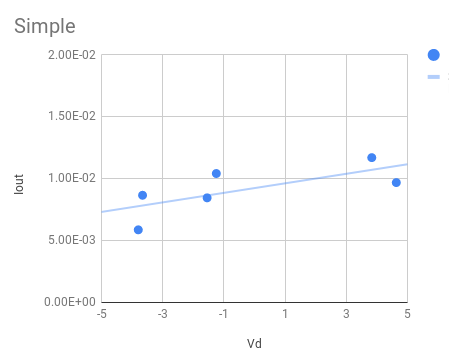
\includegraphics[width=4.0 in]{simple_rout.png}
		\caption{Simple current source $V_o$ vs. $I_D$}
		\label{fig:simple_r}
	\end{figure}

	\begin{figure}[H]
		\centering
		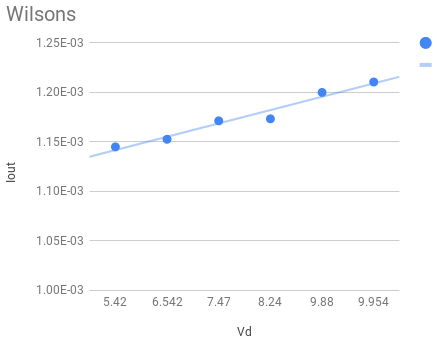
\includegraphics[width=4.0 in]{wilson_rout.png}
		\caption{Modified Wilson current source $V_o$ vs. $I_D$}
		\label{fig:wilson_r}
	\end{figure}

	\begin{table}[H]
		\centering
		\caption{Experimental $R_{out}$}
		\label{table:rout}
		\begin{tabular}{|c|c|}
			\hline
			Current Source & $R_{out}$\\
			\hline
			Simple & 38.5 $\si{\kilo\ohm}$\\
			Wilson & 1.3 $\si{\mega\ohm}$\\
			\hline
		\end{tabular}
	\end{table}
	
	These experimentally found values for $R_{out}$ are relativley close to
	the values calculated in the Theory section and again shows that the
	modified Wilsons current source has a significantly higher output
	resistance.


	\section{Conclusion}
	The goal of this lab exercise was to build two different current sources,
	a simple current source and a modified Wilsons current source and measure
	their operation. The circuits were first simulated in PSPICE to verify the
	proper circuit operation, then the circuts were built in-lab and measured
	using differen load resistors. This allowed the output resistance of both
	current sources to be measured.\\

	\hfill \break

	All values found during the in-lab portion made sense and were within margin
	of error. Any differences in the experimentally found values and the values
	that were calculated can be attributed to the fact that the reference resistors
	used were not the exact calculated values. 
\end{document}
